\chapter{Les Chambres à plaques résistives de CMS}
\renewcommand\chapterillustration{RPC/rpc}
\ThisULCornerWallPaper{1}{\chapterillustration}
\minitoc

\lettrine[lines=4, slope=-0.5em]{D}{ans} ce chapitre, une description générale des chambres à plaques résistives (RPC) ainsi qu'une description détaillée des chambres RPC utilisées dans CMS et de leurs électroniques. Une description des mises à niveaux se rapportant à ces détecteurs, notamment dans les bouchons sera également présentée.

\section{Les chambres à plaques résistives (RPC)}

 \marginpar
{
	\centering
	\includegraphics[width=\marginparwidth]{RPC/Geiger.png}
	\captionof{figure}{Photo d'un des premiers tubes Geiger-Müller fabriqué en 1932 par Hans Geiger pour une utilisation en laboratoire.}
	\label{Geiger}
}
Les RPC pour \textit{Resistive Plate Chambers} font partie d'une famille de détecteurs appelé détecteurs gazeux. Ces détecteurs ont joué un rôle dès le début de la Physique des Hautes Énergies dans la détection de nouvelles particules. Depuis le premier détecteur gazeux, le compteur proportionnel à un seul fil \textit{Single-wire proportional counter} inventé par Rutherford et Geiger, puis le compteur Geiger-Müller (cf.fig~\ref{Geiger}) présenté en 1928, les détecteurs gazeux n'ont cessé de se perfectionner et de devenir plus rapide et efficaces. Ils permettent de couvrir de grandes surfaces de détections à des coûts très modestes.

\subsection{Les détecteurs gazeux}
Les détecteurs gazeux reposent tous sur le même principe simple. Lorsqu'une particule traverse un gaz, elle l'ionise. Les ions et électrons créés lors de cette ionisation peuvent être accélérés grâce à un champ électrique. En choisissant judicieusement l'intensité du champ électrique, c'est à dire en appliquant une tension aux bornes des électrodes, les électrons peuvent gagner assez d'énergie pour ioniser le gaz à leur tour (seconde ionisation) et commencer une multiplication de charge. Le nombre de charges libérées détermine le mode de fonctionnement du détecteur. Le gaz est également un élément important du détecteur et a un rôle important sur le mode de fonctionnement de celui-ci. Le déplacement des charges à l'intérieur du gaz induit un déplacement de charges sur les électrodes, et crée un signal qui peut être récupéré par une électronique et donner une information sur le temps et la position de la trajectoire de la particule incidente. Ces charges peuvent donner lieu à un mode dit "streamer" voire donner lieu à la création d'étincelles entre l'anode et la cathode. La figure \ref{mult} montre le facteur d'amplification, ou le gain du gaz en fonction du voltage appliqué. 

\begin{figure}[ht!]
	\centering
	\includegraphics[width=0.95\textwidth]{RPC/gasgain.png}
	\captionof{figure}{Évolution typique de gain du gaz en fonction du voltage appliqué (en échelle arbitraire).}
	\label{mult}
\end{figure}

Six régions peuvent être définies :

\begin{itemize}
	\item \textbf{I} Les paires d'électrons-ions primaires se recombinent avant d'avoir été toutes récoltées.
	\item \textbf{II} Les charges dues à l'ionisation primaire sont entièrement récoltées sur les électrodes. Le facteur d'amplification reste constant même si le voltage est augmenté.
	\item \textbf{III} Les charges produites par l'avalanche sont proportionnelles aux charges produites lors de la première ionisation. Les charges collectées augmentent fortement avec la tension appliquée.
	\item \textbf{IV} Cette région est la limite de proportionnalité, l'avalanche se transforme en streamer, un plasma d'ions et d'électrons.
	\item \textbf{V} Les streamers connectent les électrodes et produisent des étincelles visibles. Les compteurs Geiger-Müller et les chambres à étincelles fonctionnent dans ce mode.
	\item \textbf{VI} Des décharges électrique se produisent même sans le passage de particules pour ioniser le gaz. Ce mode peut détruire le détecteur.
\end{itemize}

Les détecteurs gazeux à fils ont une résolution temporelle de l'ordre de la centaine de nanoseconde. Cela est dû au champ électrique en $\frac{1}{r}$, qui fait que la zone d'amplification se situe proche du fil et les électrons doivent atteindre cette zone avant d'être amplifiés et de démarrer l'avalanche.

En utilisant un champ électrique uniforme et important, une meilleure résolution temporelle est atteignable.

Le premier détecteur gazeux utilisant cette méthode est le compteur à étincelle "Spark Counter" développé dans les années 1948, un détecteur qui présente une géométrie plane. Il est généralement constitué de deux électrodes métalliques entre lesquelles est présent un gaz. Le passage d'une particule ionise ce gaz et crée une avalanche qui rentre à un certain moment en mode streamer. Un plasma se crée entre les deux électrodes, les électrodes se déchargent et amènent à la création d'une étincelle. Ce type de détecteur présente un signal qui ne nécessite pas d'amplification, cependant le temps nécessaire à la recharge des électrodes est de l'ordre de quelques millisecondes. De plus la surface du détecteur ne doit pas être trop grande ($\sim$\SI{10}{\square\centi\meter}) afin de ne pas détruire les électrodes lors des décharges.

Afin de résoudre ces problèmes, les électrodes métalliques peuvent être remplacées par des plaques de matériaux de haute résistivité (\SIrange{10e9}{10e10}{\ohm\centi\meter}) afin de limiter l'aire de décharge des électrodes autour du signal. Un mélange de gaz absorbant les photons permet d'éviter le mode streamer. Ce qui permet le fonctionnement du détecteur à des flux de particules plus important. Le champs électrique baissant localement du fait de la recharge plus lente des électrodes, le développement d'avalanches successives au même endroit est limité tout en laissant le détecteur opérationnel hors de cette zone.
\vspace{-0.3cm}
\subsubsection{Naissance des RPC}
\vspace{-0.3cm}
En 1981 R.Santonico et R.Cardarelli développent les Resistive Plate Chamber (RPC) \cite{Santonico:1981sc} \cite{CARDARELLI198820}. Ce détecteur utilise un matériau peu coûteux, très utilisé et de haute résistivité ($\sim$\SI{e10}{\ohm\centi\meter}), le High Pressure Laminate (HPL) fait de mélamine ou un type de résine phénol-formaldéhyde (anhydrure de polyoxybenzylméthylèneglycol ou Bakélite (cf.fig~\ref{bakelite})). 
\marginpar
{
	\centering
	\includegraphics[width=\marginparwidth]{RPC/bakelite.png}
	\captionof{figure}{Structure de la Bakélite.}
	\label{bakelite}
}
Plusieurs configuration pour les RPC sont possibles, mais l'une des plus simples est donnée par la figure \ref{RPCscheme}.

\begin{figure}[th!]
	\centering
	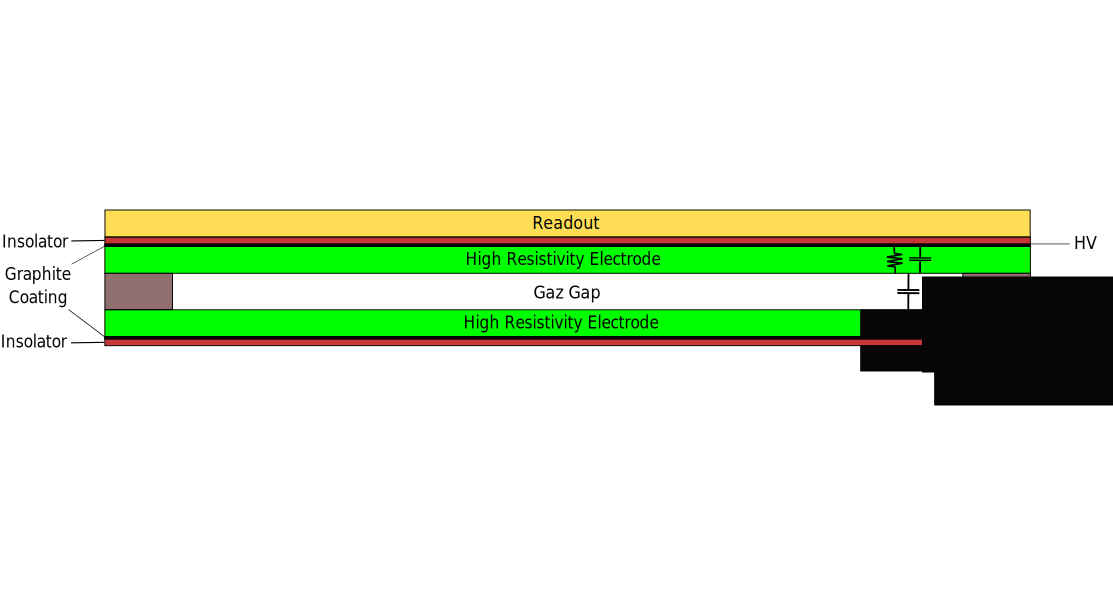
\includegraphics[width=0.98\textwidth]{RPC/scheme_first.png}
	\captionof{figure}{Schéma d'une RPC typique.}
	\label{RPCscheme}
\end{figure}
\vspace{-0.1cm}
Une couche de gaz est comprise entre deux plaques d'électrodes résistives. Ces plaques sont peintes avec du graphite qui est utilisé pour distribuer la haute tension sur les électrodes. L'électronique est isolée de la chambre par un isolant fin, de type feuille de poly(téréphtalate d'éthylène) (Mylar). L'électronique peut être placée de chaque coté de la chambre et peut être constituée de carreaux ou de lamelles etc.

Un modèle électrique simplifié d'un RPC peut être obtenu (cf.ref~\ref{RPCscheme}). En notant, $C_{b}$ la capacité de la bakélite, $R_{b}$ sa résistance et $C_{g}$ la capacité du gaz.

La résistance de la bakélite est donnée par :
\begin{equation}
R_b=\frac{\rho d}{S}
\end{equation}
avec $\rho$ la résistivité de la bakélite, $d$ l'épaisseur de l'électrode et $S$ sa surface.

La capacité de la bakélite est donnée quant à elle par :
\begin{equation}
C_{b}=\epsilon_0\epsilon_r\frac{S}{d}
\end{equation} 
avec $\epsilon_0$ la permittivité du vide et $\epsilon_r$ la permittivité relative de la Bakélite.

Le temps de décharge d'une électrode de telle résistivitéet capacité recevant une charge $Q_{0}$ est donné par :
\begin{equation}
Q(t)=Q_{0}e^{\frac{-t}{R_bC_b}}=Q_{0}e^{\frac{-t}{\rho\epsilon_{0}\epsilon_{r}}}=Q_{0}e^{\frac{-t}{\tau}}
\end{equation}
Les charges présentes sur les électrodes réduisent la haute tension appliquée et donc le champ électrique à l'endroit des charges. Le détecteur devient inefficace pour cette période de temps $\tau$ à l'endroit du dépôt des charges tout en restant efficace ailleurs. Pour le cas de la bakélite $\rho\simeq\SI{10e10}{\ohm\centi\meter}$ le temps de relaxation est de l'ordre de \SI{10}{\micro\second}. Grâce à l'utilisation de matériaux de haute résistivité, l'utilisation de chambres de grande taille était désormais possible.


Depuis, ces détecteurs de construction simple et robuste ont été utilisés dans de nombreuses expériences : ATLAS \cite{ATLAS}, BaBar \cite{Boutigny:1995ib} (cf.fig~\ref{babar}), BELLE \cite{ABASHIAN2002117} (cf.fig~\ref{belle}),  Oscillation Project with Emulsion-tRacking Apparatus (OPERA) \cite{1748-0221-9-10-C10003} (cf.fig~\ref{opera}) etc. Différentes solutions technologiques ont été développées selon les besoins des différentes expériences.

\marginpar
{
	\centering
	\includegraphics[width=\marginparwidth]{RPC/babar.png}
	\captionof{figure}{Schéma de l'expérience BaBar.}
	\label{babar}
}

\marginpar
{
	\centering
	\includegraphics[width=\marginparwidth]{RPC/belle.png}
	\captionof{figure}{Schéma de l'expérience BELLE.}
	\label{belle}
}

\marginpar
{
	\centering
	\includegraphics[width=\marginparwidth]{RPC/OPERA.jpg}
	\captionof{figure}{Photo du détecteur OPERA.}
	\label{opera}
}

\subsection{Principes de fonctionnement d'une RPC}
Le principe d'une RPC repose sur l'ionisation d'un gaz. Lorsqu'une particule relativiste traverse le gaz d'une RPC, elle interagit avec les molécules de gaz principalement par interaction électromagnétique. La perte d'énergie moyenne par ionisation et excitation d'une particule relativiste massive ($m>m_{e}$) due à des électrons libres supposés au repos est donnée par la formule de Bethe-Bloch (cd.fig\ref{Bethe-Block})
\begin{equation}
-\left<\frac{1}{\rho}\frac{\dd E}{\dd x}\right>=\frac{e^{4}}{4\pi \epsilon_{0}^{2}m_{e}c^{2}}z^{2}N_{A}\frac{Z}{A}\frac{1}{\beta^{2}}\left[\frac{1}{2}\ln\frac{2m_{e}c^{2}\beta^{2}\gamma^{2}E_{max}}{I^{2}}-\beta^{2}-\frac{\delta(\beta\gamma)}{2}\right]
\end{equation}
avec :

\begin{itemize}[label=$\bullet$]
	\item $\rho$ la densité du matériau,
	\item $e$ la charge de l'électron,
	\item $\epsilon_{0}$ la permittivité du vide,
	\item $c$ la vitesse de la lumière dans le vide,
	\item $z$ la charge de la particule incidente,
	\item $N_{A}$ le nombre d'Avogadro,
	\item $Z$ le numéro atomique du matériau,
	\item $A$ le nombre de masse du matériau,
	\item $\beta=\frac{v}{c}$ la vitesse de la particule incidente en unité de $c$,
	\item $\gamma=\frac{1}{\sqrt{1-\beta^{2}}}$
	\item $I$ est l'énergie d'excitation moyenne et
	\item $E_{max}$ est l'énergie maximale transférée lors d'une collision d'une particule de masse $m$ et de quantité de mouvement $p$,
	\begin{equation}
	E_{max}=\frac{2m_{e}p^{2}}{m^2+2\gamma m_{e}m+m_{e}^2}
	\end{equation}
\end{itemize}

\begin{minipagewithmarginpars}[h]{0.95\textwidth}
	\centering
	\includegraphics[width=0.70\textwidth]{RPC/Bethe-Bloch.eps}
	\captionof{figure}{Perte d'énergie moyenne $-\left<\frac{\dd E}{\dd x}\right>$ pour des anti-muons dans du cuivre en fonction de $\beta\gamma=\frac{p}{Mc}$ sur neuf ordres de grandeurs en quantité de mouvement (12 ordres de grandeurs en énergie cinétique)\cite{Olive:2016xmw}.}
	\label{Bethe-Block}
\end{minipagewithmarginpars}

\marginpar
{
	\centering
	\includegraphics[width=\marginparwidth]{RPC/Photon.png}
	\captionof{figure}{Émission d'un photon lors de la désexcitation d'un atome.}
	\label{photon}
}
\marginpar
{
	\centering
	\includegraphics[width=\marginparwidth]{RPC/Auger.png}
	\captionof{figure}{Éjection d'un électron Auger.}
	\label{Auger}
}
\marginpar
{
	\centering
	\includegraphics[width=\marginparwidth]{RPC/Penning.png}
	\captionof{figure}{Ionisation Penning.}
	\label{Penning}
}
\marginpar
{
	\centering
	\includegraphics[width=\marginparwidth]{RPC/Brem.png}
	\captionof{figure}{Bremsstrahlung produit par un électron dévié par le champ électrique d'un noyau.}
	\label{Brem}
}

Si un atome ou une molécule du gaz est ionisé par la collision inélastique de la particule incidente, des électrons sont éjectés de l'atome près du point de collision. En revanche, si l'atome n'est pas ionisé mais excité, l'énergie d'excitation est évacuée par l'émission d'un photon (cf.fig~\ref{photon}), par un électron Auger (cf.fig~\ref{Auger}) ou par ionisation Penning (cf.fig~\ref{Penning}). Si ce photon a une énergie plus importante que le minimum du potentiel d'ionisation, le photon va être absorbé par effet photoélectrique et un électron va être éjecté de l'atome, sinon le photon ne sera pas détecté par les RPC.

Une particule chargée relativiste peut aussi perdre son énergie par rayonnement continu de freinage appelé \textit{Bremsstrahlung}(cf.fig~\ref{Brem}), ce processus devient prédominant si l'énergie de la particule dépasse une certaine énergie critique ($E_{\mu c}$ sur la figure \ref{Bethe-Block}). Dans ce cas, la perte d'énergie n'est pas détectée par le RPC.

Le fonctionnement d'une RPC repose sur la perte d'énergie par ionisation et excitation. Cette perte d'énergie dépend du matériau (cf.fig~ \ref{mat}). Lors de l'ionisation du gaz, des amas primaires (d'électrons et ions) sont créés le long de la trajectoire de la particule incidente. 


\begin{figure}[ht!]
	\centering
	\includegraphics[width=0.55\textwidth]{RPC/energylost.png}
	\captionof{figure}{Perte d'énergie moyenne dans l'hydrogène liquide, l'hélium liquide, le carbone, l'aluminium, le fer, l'étain et le plomb. Les effets radiatifs, pertinents pour les pions et muons ne sont pas inclus. Ils deviennent importants pour les muons traversant le fer avec $\beta\gamma\gtrsim1000$ et à plus petite quantité de mouvement pour les muons dans des absorbeurs de plus grand $Z$.\cite{Olive:2016xmw} }
	\label{mat}
\end{figure}

\subsection{Les modes de fonctionnement des RPC}

Selon l'intensité du champ électrique appliqué  entre les électrodes, il est possible de choisir le mode de fonctionnement des chambres. La composition du mélange gazeux est également un élément déterminant. On distingue généralement trois modes de fonctionnement; le mode avalanche, le mode streamer et éclair (Spark).

\subsubsection{Le mode avalanche}

Le mode avalanche est le premier mode de fonctionnement qui apparait lorsqu'on augmente la tension entre les électrodes. L'ionisation du gaz crée quelques paires d'ion-électrons qui sont ensuite accélérées par le champ électrique. Les électrons, qui sont beaucoup plus rapides que les ions de par leur masse plus faible vont à leur tours ioniser les molécules du gaz. Cette multiplication des charges est appelée avalanche. Ce déplacement va créer par effet capacitif un signal de l'ordre de la nanoseconde qui peut être récolté. Les charges vont ensuite atteindre les électrodes et s'y accumuler, et vont être neutralisées en quelques millisecondes grâce au courant fourni par le générateur de haute tension appliquant la différence de potentiel (cf.fig~\ref{avalanche}). Le temps mort de ce mode est donc assez faible et permet donc une détection efficace des particules mêle à des flux assez elevée($\sim\SI{1}{\kilo\hertz}$), la résistivité du matériaux est déterminante pour ce temps de neutralisation des charges. Cependant, la charge induite est faible et nécessite donc une électronique possédant un bas seuil et donc de bas bruit.

\begin{figure}[ht!]
\centering
\subfloat[Des molècules du gaz sont ionisées par le passage d'une particule.]{\includegraphics[width=.49\linewidth]{RPC/avalanche-streamer-1.png}\label{avalanche-1}}
\hfill
\subfloat[La taille de l'avalanche influence le champ électrique local de la couche de gaz.]{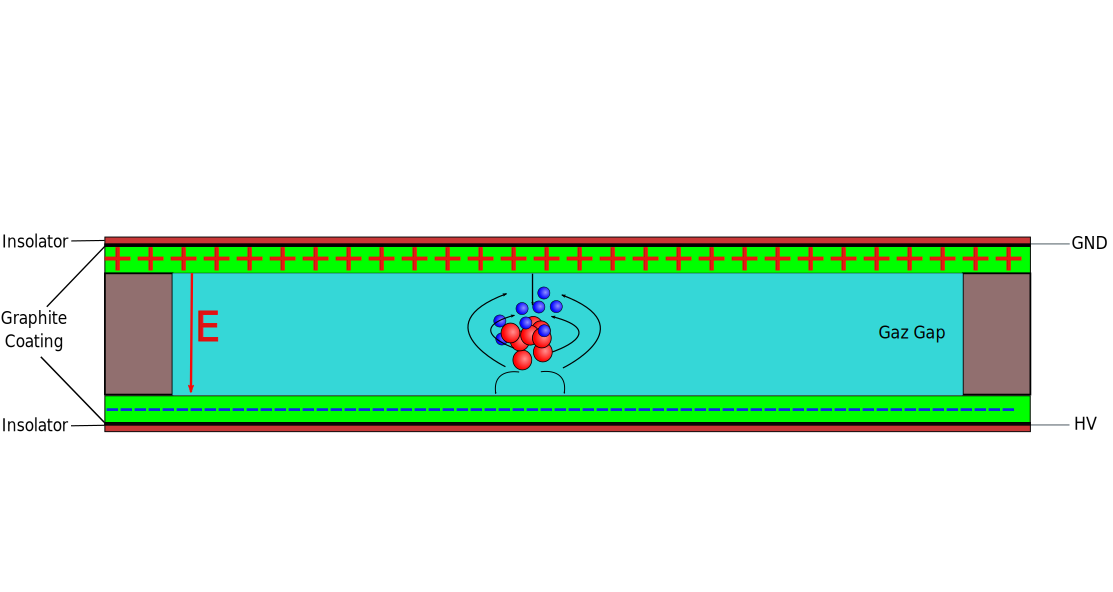
\includegraphics[width=.49\linewidth]{RPC/avalanche-2.png}\label{avalanche-2}}
\\
\subfloat[Les électrons atteignent l'anode. Les ions sont beaucoup plus lent ]{\includegraphics[width=.49\linewidth]{RPC/avalanche-3.png}\label{avalanche-3}}
\hfill
\subfloat[Les ions atteignent la cathode. Les charges de la couche résistive induisent un temps mort.]{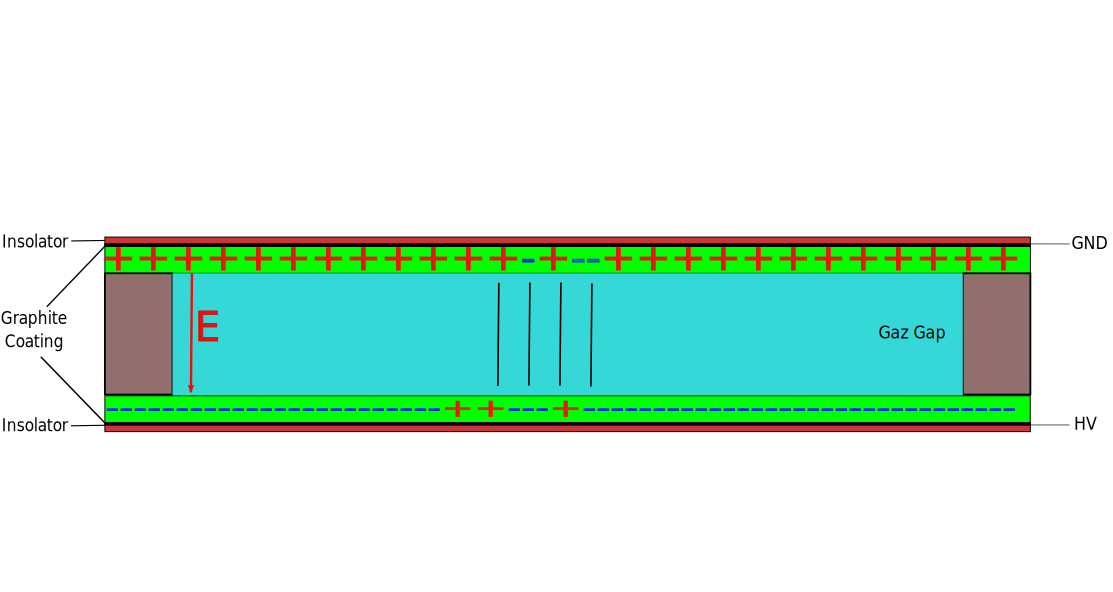
\includegraphics[width=.49\linewidth]{RPC/avalanche-4.png}\label{avalanche-4}}
\caption{Vue schématique du développement d'une avalanche. Le champ électrique appliqué aux électrodes est noté $E$, les électrons sont en bleu et les ions en rouge.}
\label{avalanche}
\end{figure}

\subsubsection{Le mode streamer}

Si l'on augmente la tension aux bornes des électrodes, le gain du gaz augmente, les ionisations primaires créent donc plus d'ionisations secondaires, il y'a donc création de paires électrons-ions  en plus grand nombre. De plus les photons peuvent commencer à contribuer à la propagation de l'avalanche, ce qui amène au mode streamer. Le signal engendré par ce mode est plutôt important (de 50pC à quelques nC), l'électronique peut donc se passer d'amplification et est donc beaucoup plus simple. Cependant, le flux de particules maximal est limité à quelques centaines de hertz. Si le nombre d'électrons devient trop important (en moyenne $10^{8}$ électrons), ils engendrent la création d'un plasma reliant les deux électrodes (cf.fig~ \ref{streamer}).

\begin{figure}[ht!]
	\centering
	\subfloat[Des molècules du gaz sont ionisées par le passage d'une particule.]{\includegraphics[width=.49\linewidth]{RPC/avalanche-streamer-1.png}\label{streamer-1}}
	\hfill
	\subfloat[La taille de l'avalanche modifie fortement le champ électrique local de la couche de gaz. ]{\includegraphics[width=.49\linewidth]{RPC/streamer-22.png}\label{streamer-2}}
	\\
	\subfloat[les photons contribuent au développement de l'avalanche et étalent l'avalanche. Passage au mode streamer]{\includegraphics[width=.49\linewidth]{RPC/streamer-3.png}\label{streamer-3}}
	\hfill
	\subfloat[Les charges de la couche Résistive induisent un temps mort important.]{\includegraphics[width=.49\linewidth]{RPC/streamer-5.png}\label{streamer-5}}
	\caption{Vue schématique du développement d'un streamer. Le champ électrique appliqué aux électrodes est noté $E$, les électrons sont en bleu et les ions en rouge.}
	\label{streamer}
\end{figure}

\subsubsection{Le mode éclair (Spark)}
Si l'on augmente encore la tension ou si le mélange de gaz ne permet pas de limiter la propagation latérale de l'avalanche ou le mode streamer, les électrons migrateurs et les photons peuvent induire de proches en proches d'autres streamers, c'est le mode éclair, ou Spark. Les éclairs se propagent alors dans toute la chambre. Le temps de recouvrement de la chambre est alors très long et les charges accumulé peuvent détériorer rapidement le détecteur. De plus le flux de particules détectable est très faible (cf.fig~ \ref{spark}).
\begin{figure}[ht!]
	\centering
	\subfloat[Des molècules du gaz sont ionisées par le passage d'une particule.]{\includegraphics[width=.49\linewidth]{RPC/avalanche-streamer-1.png}\label{spark-1}}
	\hfill
	\subfloat[La taille de l'avalanche modifie fortement le champ électrique local de la couche de gaz. ]{\includegraphics[width=.49\linewidth]{RPC/spark-2.png}\label{spark-2}}
	\\
	\subfloat[les photons contribuent au développement de l'avalanche et étalent l'avalanche. Passage au mode streamer]{\includegraphics[width=.49\linewidth]{RPC/streamer-3.png}\label{spark-3}}
	\hfill
	\subfloat[Un plasma peut se créer entre les électrodes et créer une étincelle. Les electrodes sont déchargées à cet endroit (mode éclair).]{\includegraphics[width=.49\linewidth]{RPC/streamer-4.png}\label{spark-4}}
    \\
	\subfloat[Des éclairs se créent de proche en proche à cause des électrons migrateurs et des photons.]{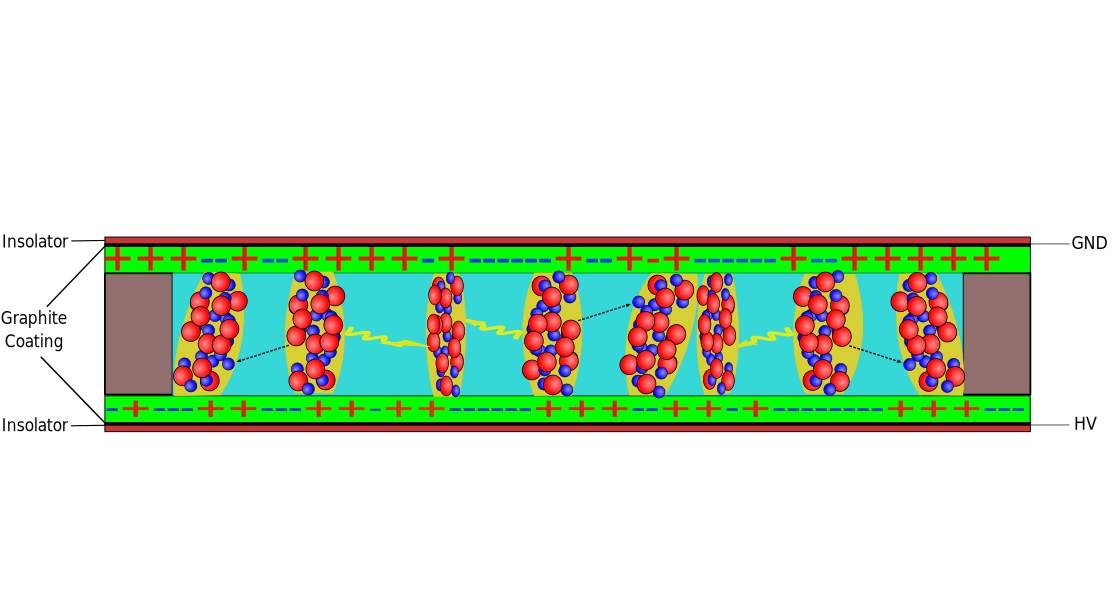
\includegraphics[width=.49\linewidth]{RPC/spark-5.png}\label{spark-5}}
    \hfill
	\subfloat[Le champ électrique est fortement baissé dans toute la chambre; Elle est aveugle.]{\includegraphics[width=.49\linewidth]{RPC/spark-6.png}\label{spark-6}}
	\caption{Vue schématique du développement d'un spark. Le champ électrique appliqué aux électrodes est noté $E$, les électrons sont en bleu et les ions en rouge.}
	\label{spark}
\end{figure}


Dans CMS le mélange de gaz ainsi que les tensions appliquées ont été judicieusement étudiées pour que les RPC soient le plus possible en mode avalanche afin de maximiser le flux de particules que peut détecter les chambres ainsi que d'éviter un vieillissement prématuré de ces chambres. C'est donc ce mode que nous allons étudier plus en avant.

\subsection{Étude théorique du mode avalanche}

\subsubsection{Ionisation primaire}
Le mélange gazeux des détecteurs contient majoritairement un gaz à faible potentiel d'ionisation minimale afin d'être facilement ionisable. En pratique, la plupart des détecteurs utilisent du TFE de potentiel d'ionisation minimal $U_{i}=\SI{10.114 \pm0.010}{\eV}$ \cite{Chimie:chimie}. La création de charges primaires dues au passage d'une particule chargée dans le mélange de gaz est caractérisée par le nombre moyen d'amas créés par unité de longueur ainsi que par le nombres de paires d'électron-ions créées dans chaque amas.

\subsubsection{Distance entre les amas de l'ionisation primaire}
Si l'on considère que l'énergie perdue dans le matériau par la particule incidente est négligeable par rapport à son énergie alors les probabilités de collisions ionisantes sont indépendantes. Les distances entre les amas d'ionisations primaires suivent donc une loi exponentielle :
\begin{equation}
P(z)=\frac{1}{L}\exp\left(-\frac{z}{L}\right)
\end{equation} 
où $L$ est le libre parcourt moyen et z l'épaisseur à laquelle l'ionisation à lieu en considérant des particules incidentes dont la trajectoire est normale au plan du détecteur. Pour des particule incidente d'angle $\phi$ par rapport à l'axe z la formule devient:
\begin{equation}
P(z)=\frac{1}{L}\exp\left(-\frac{z}{L\cos\phi}\right)
\end{equation}
La distance moyenne entre amas primaires peut se calculer en utilisant le programme de simulation Monte-Carlo HEED \cite{HEED}. Une comparaison entre les mesures et les simulations pour l'isobutane et le méthane est donnée fig\ref{lambda} et montre de bon accord \cite{2004NIMPA}.  

\begin{figure}[ht!]
	\centering
	\includegraphics[width=0.60\textwidth]{RPC/lambda.png}
	\captionof{figure}{Nombre de collisions donnant lieux à des ionisations (nombre d'amas) par \si{\milli\meter} en function de $\gamma-1$, $\gamma=\frac{1}{\sqrt{1-\beta^{2}}}$ pour différents mélanges de gaz, prédit par HEED. $T=$\SI{296.15}{\kelvin} et $p=$\SI{1013}{\milli\bar}. Les lignes correspondent à des mesures prises de \cite{PhysRevA.6.1507}.  }
	\label{lambda}
\end{figure}

Le nombre moyen d'amas contenus dans une couche de gaz d'épaisseur $e$ est donc $\bar{n}=\frac{e}{L}$. La probabilité d'avoir $n$ amas dans cette couche de gaz suit une loi de Poisson :
\begin{equation}
P(n)=\frac{1}{n!}\left(\frac{e}{L}\right)^{n}\exp\left(-\frac{e}{L}\right).
\end{equation}
En supposant un détecteur parfait, l'efficacité maximale pour une chambre d'épaisseur $e$ est donnée par :
\begin{equation}
\epsilon_{max}=1-P(0)=1-\exp\left(-\bar{n}\right)
\end{equation}
où $P(0)$ est la probabilité qu'aucune ionisation ne soit créée dans l'épaisseur de gaz de la chambre.

\subsubsection{Nombre d'électrons dans les amas primaires}
Le nombre d'électrons par amas d'ionisation primaire est variable et dépend de l'énergie échangée entre le gaz et la particule incidente. La distribution du "cluster size" a été calculée par Riegler et al. \cite{Riegler:570462} en utilisant HEED pour des mélanges de gaz très utilisés pour les RPC (cf.fig~\ref{cluster})
\begin{figure}[ht!]
	\centering
	\includegraphics[width=0.60\textwidth]{RPC/cluster.png}
	\captionof{figure}{Distributions du "cluster size" pour un mélange gazeux typique utilisé pour les RPC calculées en utilisant HEED. Les particules incidentes sont des pions de \SI{7}{\giga\eV} pour le mélange avec 10\% d'isobutane et \SI{120}{\giga\eV} pour le mélange avec 0.3\%. La température du gaz est $T=$\SI{296.15}{\kelvin} et la pression $p=$\SI{1013}{\milli\bar}. En coupant à 500 électrons et par intégration on trourve un nombre d'électron moyen par amas de 1.9 pour l'isobutane, 2.6 pour le mélange à 10\% de \chemform{SF_6} et 2.8 pour le mélange à 0.3\% de \chemform{SF_6}.}
	\label{cluster}
\end{figure}

\subsection{Le facteur de multiplication}
Après l'ionisation, les électrons primaires vont être accélérés grâce au champ électrique entre les électrodes ce qui peut donner lieu à une avalanche. Cependant afin d'éviter les modes streamer et spark, le mélange gazeux contient généralement des gaz très électronégatifs ce qui à pour effet de capturer certains électrons primaires, les molécule très électronégatives ayant tendance à vouloir former des anions, et de réduire ainsi la taille de l'avalanche. 

Tous les électrons non absorbés sont accélérés par le champ électrique et sont soumis à des chocs élastiques et inélastiques avec les autres molécules du gaz. Si l'énergie échangée lors de ces collisions est assez importante pour ioniser à son tour d'autres molécules du gaz, on assiste à une multiplication des paires électron-ion et à une réaction en cascade. Les électrons migrent vers l'anode et les cations vers la cathode mais à des vitesses beaucoup moins élevées que pour les électrons de par leur masse beaucoup plus importante. Ces processus ont de très grandes fluctuations stochastiques.

En définissant $\alpha$ le taux de création de paires d'ion-électron secondaires créées par unité de distance (coefficient d'ionisation de Townsend) et  $\beta$ le taux d'électrons capturés par unité de distance par les molécules électronégatives pour former des anions (coefficient d'attachement), il vient pour un déplacement  $\dd z$.
\begin{equation}
	\frac{\dd \bar{n}}{\dd z}=(\alpha-\beta)\bar{n} \quad  \frac{\dd \bar{p}}{\dd z}=\alpha\bar{n} 
\end{equation}
avec la première équation décrivant la variation du nombre moyen d'électrons et la deuxième celle du nombre moyen d'ions positifs. On peut définir également $\alpha_{eff}=\alpha-\beta$ qu'on appelle coefficient de Townsend effectif. En posant les conditions initiales $\bar{n}=1$ et $\bar{p}=0$, on obtient les nombres moyens d'électrons et d'ions positifs produits sur une distance $x$: 
\begin{equation}
\bar{n}=\exp(\alpha-\beta)z \quad \bar{p}=\frac{\alpha}{\alpha-\beta}\left(\exp^{(\alpha-\beta)z}-1\right)
\end{equation}
Le coefficient de Townsend dépend du champ électrique appliqué. La figure \ref{tow} montre cette dépendance pour un mélange de gaz.

\begin{figure}[ht!]
	\centering
	\includegraphics[width=0.62\textwidth]{RPC/tow.png}
	\captionof{figure}{Coefficient de Townsend et coefficient d'attachement calculés grâce à Imonte \cite{imonte} pour $T=296.15K$ et $p=1013mbar$ pour un mélange de gaz particulier \cite{Riegler:570462}. }
	\label{tow}
\end{figure}

\subsection{Charges créées par l'avalanche}
La charge totale à la fin du développement du processus de multiplication peut être vue comme la somme de plusieurs avalanches qui sont indépendantes l'une de l'autre. Chaque amas primaire crée son avalanche qui est soumise à des fluctuations statistiques.

En supposant $\alpha$ et $\beta$ constantes, la charge totale à l'emplacement $z$ peut être exprimée comme :
\begin{equation}
q(z)=\sum_{j=1}^{n_c}q_{e}M_{j}n_{j,0}\exp^{(\alpha-\beta)(z-z_O^j)}
\end{equation}
\newpage
Les fluctuations statistiques sont prises en compte par 4 variables aléatoires :
\begin{itemize}[label=$\bullet$]
	\item Le nombre d'amas $n_c$ qui suit une distribution poissonienne 
	\begin{equation}
	P_{clusters}(n_c=n)=\frac{(\lambda_{eff}d)^{n}}{n!}\exp^{-\lambda_{eff}d}
	\end{equation}
	avec $\lambda_{eff}=\frac{\lambda}{\phi}$ la densité linéaire moyenne d'amas, $\phi$ l'angle d'incidence de la particule incidente et d l'épaisseur de la couche de gaz.
	\item La position $z_0^j$ du cluster $j$ suit la loi Gamma
	\begin{equation}
	P_{j}(z_0^j=x)=\frac{x^{j-1}\lambda_{eff}^{j}}{\Gamma(j)}\exp^{-x\lambda_{eff}} \quad 0<x<d
	\end{equation}
	\item Le nombre d'électrons $n_{0}^{j}$ dans le cluster $j$ suit la loi de distribution trouvé par le programme Heed (cf.fig~\ref{cluster}) 
	\item Le facteur $M_{j}$ qui prend en compte les fluctuations de l'avalanche et la diminution par les ions lorsque l'avalanche devient trop importante du champ électrique réduit $E/p$ avec $p$ la pression du gaz . Ce facteur est obtenu concrètement en tirant d'une distribution de Polya une valeur puis en la divisant par le nombre moyen d'électrons de l'avalanche.
\end{itemize}
\vspace*{-0.2cm}
\subsection{Signal induit sur l'électronique}
\vspace*{-0.6cm}
En utilisant le théorème de Ramo et Shockley \cite{HE2001250}, il peut être montré que le courant électrique induit sur l'électronique est dû au mouvement des charges entre les électrodes qui change les lignes de champ électrique et non la quantité de charge reçue par seconde par l'électrode. C'est ce courant qui peut ensuite être traité par l'électronique de lecture.
\begin{equation}
i_{ind}(t)=-q(x/v_{d})\vec{v_{d}}\cdot \vec{E_{w}}
\end{equation}
où $\vec{E_{w}}$ est appelé le champ pondéré et correspond au champ électrique du détecteur si la charge est enlevée, l'électrode mise à une tension unitaire  et toutes les autres électrodes sont mises à la masse. $\vec{v_{d}}$ est la vitesse de dérive des charges.

La vitesse de dérive pour les électrons dans différents mélanges de gaz est donné sur la figure \ref{drift} \cite{Riegler:570462}

\begin{figure}[ht!]
	\centering
	\includegraphics[width=0.60\textwidth]{RPC/drift.png}
	\captionof{figure}{Vitesse de dérive calculé en utilisant le programme MAGBOLTZ \cite{MAGBOLTZ} pour différents mélanges de gaz à la température $T=$\SI{296.15}{\kelvin} et pression $p=$\SI{1013}{\milli\bar}.}
	\label{drift}
\end{figure}

De par leur masse beaucoup plus élevée que les électrons, les ions se déplacent plus lentement et participent moins au courant induit, ils mettent en revanche plus de temps pour atteindre l'électrode, le signal induit est donc beaucoup plus long et accroit le temps mort du détecteur.

\section{Les Resistive Plate Chambers de CMS}

Le détecteur CMS utilise des chambres double gaps d'épaisseur \SI{2}{\milli\meter}, chacun formés par deux électrodes en Bakélite de résistivité comprise entre \SI{1e10}{\ohm\centi\meter} et \SI{6e10}{\ohm\centi\meter} (cf.fig\ref{cmsrpc}). 

\begin{figure}[ht!]
	\centering
	\includegraphics[width=0.90\textwidth]{RPC/CMSRPC.png}
	\captionof{figure}{Schèma d'une chambre RPC dans CMS.}
	\label{cmsrpc}
\end{figure}

Afin de maintenir la distance de \SI{2}{\milli\meter} entre les électrodes, des spacers en Polychlorure de vinyle (PVC) de \SI{8}{\milli\meter} de diamètre sont placés tous le \SI{10}{\centi\meter}. Les faces externes des électrodes sont recouverte d'une peinture de graphite de résistance surfacique $\approx$\SI{e5}{\ohm\per\sq} permettant la mise sous tension des chambres. Un film l'huile de lin d'épaisseur \SIrange{35}{45}{\micro\meter} est apliquée sur les faces constituant les parties internes des gaps afin d'améliorer la planéité des surfaces \cite{oil} et limiter les photons ultra-violet \cite{Lu:2009zzd}, ce qui a pour effet  de réduire le bruit et le courant de fuite des RPC.
Le signal est récolté par des strips placé entre les deux chambres et séparé de celle-ci par une couche de Mylar. Les chambres opérent en mde avalanche pour les raisons déjà évoquées dans ce chapitres.

\subsection{Le mélange gazeux}
Le mélange gazeux utilisé par les RPC de CMS comporte :
\marginpar
{
	\centering
	\includegraphics[width=\marginparwidth]{RPC/C2H2F4.png}
	\captionof{figure}{Structure chimique du Tétrafluoroéthane.}
	\label{Tetra}
}
\marginpar
{
	\centering
	\includegraphics[width=\marginparwidth]{RPC/Isobutane.png}
	\captionof{figure}{Structure chimique de l'isobutane.}
	\label{Iso}
}
\marginpar
{
	\centering
	\includegraphics[width=\marginparwidth]{RPC/Sulfurhexafluoride.png}
	\captionof{figure}{Structure chimique de l'hexafluorure de soufre.}
	\label{hexa}
}

\begin{itemize}[label=$\bullet$]
\item \num{95.2}\% de Tétrafluoroéthane \chemform{C_2H_2F_4} (R-134a) qui est le composant principal du mélange et permet une densité de cluster primaire élevé $\lambda=\SI{5.5}{\clusters\per\milli\meter}$ tout en gardant un coefficient de Townsend effectif élevé $\alpha_{eff}=\SI{9.15}{\per\milli\meter}$ \cite{CMS-NOTE-1997-004}.
\item \num{4.5}\% d'isobutane \chemform{iso-C_4H_10} qui est utilisé comme qbsorbeur de photons ultraviolet (UV) produit par la dés-excitation des molécules du mélange gazeux.
\item \num{0.3}\% d'hexafluorure de soufre \chemform{SF_6} qui est un gaz très électronégatif est permet de capturer l'excés d'électrons, il participe ainsi à augmenter le coefficient d'attachement $\beta$ et permet de réduire la probabilité de streamer \cite{Camarri:685607}.
\end{itemize}

Afin d'empêcher l'augmentation de la résistivité de la Bakélite, \num{40}\% à \num{50}\% d'humidité est ajouté au mélange gazeux \cite{Abbrescia:2004fv}.

Les gaz \chemform{C_2H_2F_4} et \chemform{SF_6} ont un  potentiel de réchauffement global (PRG) \footnote{Le PRG d’un gaz est le rapport entre les effets causés par la libération en début de période d’une masse donnée de ce gaz et ceux causés par la même masse de dioxyde de carbone (\chemform{CO_2})} \textit{Global Warming Potential (GWP)} de \num{1000} et \num{23900} sur une période de \num{100} ans. Dans le but de rejeter et de réduire la consommation de ces gaz, celui-ci circule en circuit fermé avec un une injection de gaz pur de \num{5}\% à \num{10}\% \cite{5401780}. Cependant, ces recirculation de gaz amène à l'augmentation d'impuretés comme le \chemform{HF}, le \chemform{F^-} et d'autres type de molécules à base de Fréon \cite{1748-0221-8-08-T08003}, et à une étude et un monitorage par chromatographie de la composition du gaz injecté et circulant dans les chambres. 

\subsection{Disposition des chambres RPC dans les secteurs des bouchons de CMS}
\vspace{-0.2cm}
La disposition des chambres RPC dans CMS a été présentée dans la section \ref{RPCPRE}. Ces chambres sont rectangulaires dans le tonneau et trapézoïdales dans les bouchons (cf.fig~\ref{trap}). L'aire des strips contenus dans les chambres ainsi que leur longueur ont été optimisées afin de limiter le bruit par strip qui pourrait augmenter la probabilité de coïncidences fortuites et être considéré comme le passage d'un muon. La longueur des strips est également limitée par le temps de propagation du signal le long de celui-ci. En effet, ce temps de propagation doit être plus cours que le temps de vol entre les stations. La changement de trajectoire du muon selon $\eta$ à cause du champ magnétique est également à prendre en compte pour la longueur des strips.

Les chambres sont donc divisées en deux (trois) $\eta-sectors$ pour les chambres du tonneaux (des bouchons). Les strips ont une longueur comprises entre \num{57} et \SI{125}{\centi\meter} dans le tonneau et entre \num{39.8} et \SI{79.72}{\centi\meter} dans les bouchons. Ces trois $\eta-sectors$ sont notés $A$, $B$, $C$ selon $\eta$ décroissant et comporte \num{32} strips chacun.

Cette divisions le long de $\eta$ amène à la segmentation des gaps des détecteurs afin d'extraire les signaux provenant des strips. Ainsi, les chambres des bouchons sont constitué non pas de deux mais de trois gaps noté $i$ (\textit{Bottom gap}), $ii$ (\textit{Top Wide gap}) et $iii$ (\textit{Top Narrow gap})
 (cf.fig~\ref{gapslayout}). 
\marginpar
{
	\centering
	\includegraphics[width=\marginparwidth]{RPC/schemerpc.png}
	\captionof{figure}{Schéma d'une chambre RPC dans les bouchons \cite{Tytgat:1477019}.}
	\label{trap}
}
\begin{figure}[ht!]
	\centering
	\includegraphics[width=0.50\textwidth]{RPC/gaps.png}
	\captionof{figure}{Disposition des gaps dans les chambres des bouchons \cite{gapss}.}
	\label{gapslayout}
\end{figure}

\vspace{-0.8cm}
\subsection{Électronique de lecture des chambres dans les bouchons}
\vspace{-0.2cm}
\marginpar
{
	\centering
	\includegraphics[width=\marginparwidth]{RPC/signalextraction.png}
	\captionof{figure}{Zone d'extraction des signaux.}
	\label{extraction}
}
L'électronique de lecture des signaux provenant des strips est composées de deux types de cartes :
\begin{itemize}[label=$\bullet$]
	\item Les \textbf{Front-End Boards} (FEB) (cf.fig~\ref{Feb}). Dans les bouchons, les FEB contiennent \num{4} ASIC appelées \textit{FEB Chips} s'occupant chacun de \num{8} strips qui sont connectés d'un côté grâce à des câbles coaxiaux. Le positionnement de ces FEB sur la chambre et les zones d'extraction des signaux ont été étudiés afin de limiter la gigue totale du signal (cf.fig~\ref{extraction}). Chaque chambre comporte \num{3} FEB.
	
	\begin{figure}[ht!]
		\centering
		\includegraphics[width=0.35\textwidth]{RPC/Feb.png}
		\captionof{figure}{Une Front-End Board des chambres RPC dans les bouchons de CMS. Les \num{4} ASIC sont clairement visible sur le PCB. Les strips sont connectés aux connecteurs du bas et les signaux \textit{Low-Voltage Differential Signaling} (LVDS) sont envoyé grâce aux câbles connectés aux connecteurs du haut. Le connecteur sur la droite permet la connection du FEB au \textit{Distribution Board} (DB) et amène la basse tension et les siganux I$^2$C.}
		\label{Feb}
	\end{figure}

	Le schéma de principe de l'électronique d'une voie du FEB est donné figure \ref{schemeelec} \cite{electro}, le signal est amplifié par un gain important variant linéaire $\approx$\SI{2}{\milli\volt\per\femto\coulomb} jusqu'à \SI{100}{\femto\coulomb} et un gain plus faible au delà. Un discriminateur compare ensuite le signal amplifier à un tension de seuil programmable (\SI{220}{\milli\volt} dans CMS) et permet de sélectionner la charge minimale de déclenchement, cependant ce circuit possède un time-walk de $\approx$\SI{10}{\nano\second} sur la gamme dynamique du signal d'entrée. Ce time-walk est incompatible avec l'utilisation des RPC comme système de déclenchement de CMS. Afin d'obtenir une bonne résolution temporelle en limitant le time-walk, un circuit RC différentie le signal d'entrée et l'envoie dans un zero-crossing discrimator. Ces deux signaux sont ensuite envoyé dans un circuit de coïncidence. Cette méthode permet de réduire le time-walk à $\approx$\SI{1}{\nano\second}. Le signal en sortie déclenche ensuite un circuit monostable qui définit la largeur réglable du signal de sortie. La largeur de ce signal à été réglé à $\approx$\SI{100}{\nano\second} afin de ne pas déclencher sur les rebond du signal d'entrée qui pourrait survenir étant donné qu'il n'y apas d'adaptation d'impédance au bout du strips. Finalement, le signal sort par transmission différentielle basse-tension \textit{Low-Voltage Differencial Signaling} (LVDS) grâce à des paires de câbles torsadées. Chaque FEB possède au moins un capteur de température afin de vérifier le bon fonctionnement de la carte.
	
	\begin{figure}[ht!]
		\centering
		\includegraphics[width=0.90\textwidth]{RPC/schemeelec.png}
		\captionof{figure}{Schéma de principe de l'électronique d'une voie du FEB.}
		\label{schemeelec}
	\end{figure}
	
	\item Les \textbf{Distribution Board} (DB) (cf.fig~\ref{DB}) permettent de configurer et de monitorer grâce à une interface I$^2$C les paramètres des FEB. Ces paramètres sont la tension de seuil du discriminateur (\textit{Threshold Voltage} $V_{Th}$), la largeur du signal de sortie (\textit{Monostable Voltage} $V_{Mon}$). Ces paramètre sont commun au \num{8} voies d'un même ASIC d'un FEB. Les valeurs par défaults de ces paramètres\footnote{En cas de perte de connexion} sont réglable par des potentiomètres placés sur le PCB des FEB pour les FEB servant de test. Pour les FEB présents dans les chambres de CMS, ces potentiomètres ont été remplacés par des convertisseur digital analogie (DAC). Chaque chambre des bouchons possède un DB. Les DB fournissent aussi la basse tension aux FEB.
	
		\begin{figure}[ht!]
		\centering
		\includegraphics[width=0.35\textwidth]{RPC/DB.png}
		\captionof{figure}{Un DB.}
		\label{DB}
	\end{figure}

\end{itemize}

\subsection{Point de fonctionnement des RPC}
\vspace{0.3cm}
Afin d'obtenir le meilleur point de fonctionnement pour chaque chambres RPC de CMS, des scans en tension sont effectué à chaque début du redémarrage annuel.

Les hautes tensions $H_{eff}$ sont choisit de manière équidistantes dans la gamme $[8600,9800]$ avec 
\begin{equation}
HV_{eff}(P,T)=HV\frac{P_0}{P}\frac{T}{T_0}
\end{equation}
Cette tension effective tient compte de la variation de température et de pression dans la caverne.

Ces scans sont ensuite analysés. Les courbes d'éfficacités obtenues son ajustées par une sigmoïd.

\begin{equation}
\epsilon=\frac{\epsilon_{max}}{1+e^{-\lambda\left(HV_{eff}-HV_{50\%}\right)}}
\end{equation}

Les trois paramètres de l'ajustement sont l'efficacité maximale $\epsilon_{max}$ la tension pour laquelle l'efficacité d'ajustement est égale à \num{50}\% $HV_{50\%}$ et la pente la sigmoïde au point $HV_{50\%}$, $\lambda$, définit par :

\begin{equation}
\lambda=\frac{4}{\epsilon_{max}}\frac{\dd \epsilon}{\dd \left(HV_{eff}\right)}
\end{equation}

Le point de fonctionnement $H_{work}$ est ensuite définit par $HV_{knee}+\SI{120}{\volt}$ ($HV_{knee}+\SI{100}{\volt}$) dans les bouchons (le tonneau), où $HV_{knee}$ est la tension pour laquelle l'ajustement donne une efficacité de 95\%.

La figure \ref{working} montre le point de fonctionnement moyen, l'efficacité moyenne au point de fonctionnement et la tension moyenne pour laquelle l'efficacité est de 50\% pour les différents scans en tension effectué depuis \num{2011}.
\vspace{0.5cm}
\begin{figure}[ht!]
	\centering
	\subfloat[Pour le tonneau.]{\includegraphics[width=.50\linewidth]{RPC/barrel.pdf}}
	\hfill
	\subfloat[Pour les bouchons.]{\includegraphics[width=.50\linewidth]{RPC/endcap.pdf}}
	\caption{point de fonctionnement moyen, efficacité moyenne au point de fonctionnement et la tension moyenne pour laquelle l'efficacité est de 50\% pour les différents scans en tension effectué depuis \num{2011} \cite{working2}.}
	\label{working}
\end{figure}
\newpage
\section{Mise à niveau des RPC pour la Phase-2 de CMS}
Avec la mise le passage du LHC au HL-LHC vers 2026, la luminosité est prévu pour être multiplié par à facteur \num{5} à \num{7} et le nombre d'événement pile-up devrait passé de $\approx 40$ à $\approx 140$ voir $\approx 200$. Afin de maintenir les performances de CMS, celui-ci doit également être mis à niveau. Certaines de ces améliorations ont été détallé dans le chapitre précédent.La mise à niveau du trajectographe à fait l'objet de nombreuses études compilé dans le TDR \textit{The Phase-2 Upgrade of the CMS Muon Detectors}. Les tests de vieillissement effectués montrent que la plupart des chambres du trajectographe à muons seront capable de résister à l'environnement du HL-LHC jusqu'à la fin de la Phase-2 prévu en 2038 sans une perte significative de l'éfficacité. Pour ce qui concerne les chambres RPC des bouchons, les mises à niveaux notables sont :

\begin{itemize}[label=$\bullet$]
	\item le changement du \textit{Link System} des RPC responsable d'envoyé les données des chambres RPC au système de déclenchement et au système de lecture de donnée. Le \textit{Link System} actuel possède des éléments  qui peuvent être perturbés par des bruit électromgnétique et ne sont pas certifié pour toute la durée de vie du HL-LHC. De plus le système actuelle n'enregistre les temps des hits avec une résolution temporelle de \SI{25}{\nano\second}, synchronisé avec les croisements de faisceau de CMS ce qui est un ordre de grandeur au dessus de la résolution des chambres RPC $\approx$\SI{1.5}{\nano\second}. Le nouveau système enregistrera les hits avec une résoluton de \SI{1}{\nano\second}. Cette amélioration permettra notamment de supprimer les hits de bruit arrivant hors temps, de faciliter la synchronisation du système des RPC. Un déclenchement basé sur des hypothétiques particules chargé lourdes et stables, \textit{Heavy Stable Charged Particles} (HSCP).
	
	\item L'instrumentation des régions RE3/1 et RE4/1 (cf.fig~\ref{end}) par des RPC de nouvelle générations pour les zones RE3/1 et RE4/1. Ces chambres permettrons d'étendre l'acceptance géomètrique de $|\eta|=\num{1.9}$ à  $|\eta|=\num{2.4}$. L'instrumentation de ces zones a été prévu dès le début de CMS, mais n'avait pas été réaliséà causes des flux de particules importants présents dans ces zones. 
	
	En ajoutant les chambres RPC dans les zones RE3/1 et RE4/1 au CSC déjà présent, la résolution temporelle sera amèlioré d'un facteur deux (cf.fig~\ref{intrasec}).
	
	\begin{figure}[ht!]
		\centering
		\includegraphics[width=0.90\textwidth]{RPC/intrasec.png}
		\captionof{figure}{Résolution temporelle simulée pour des traces de muons dans la région vers l'avant, dans le cas où seuls sont présents les chambres CSC et DT (bleu), et dans le cas ou les chambres RPC des zones RE3/1 et RE4/1 sont inclues.}
		\label{intrasec}
	\end{figure}
	Les nouvelles chambres RPC, \textit{improved RPC} (iRPC) auront une meilleur résolution spatiale de l'ordre de quelques centimètres le long des strips \footnote{La courbure de la trajectoire causée par le champs magnétique n'est pas pris en compte.} en utilisant un PCB permettant une lecture des strips des deux côtés. Ce type de lecture et de PCB est l'object du chapitre \ref{time} de cette thèse.
	\newpage
	Bien que les CSC peuvent identifier et déclencher sur des muons dans la région des bouchons avec une efficacité élevée, ces chambres sont moins efficaces dans certaines zone en $|\eta|$ à cause de spacers dans les chambres. En incluant les hits des RPC dans l'algorithme de recherche de segment élémentaire pour le trigger il est possible de récupérer une bonne efficacité dans ces zones (cf.fig~\ref{effii}). Il est également possible de lever les ambiguïtés des hits CSC (\textit{ghost})  au niveau du trigger L1.
	
	\begin{figure}[ht!]
	 	\centering
	 	\subfloat[Pour la station \num{3}.]{\includegraphics[width=.70\linewidth]{RPC/effstation3.png}}
	 	\\
	 	\subfloat[Pour la station \num{4}]{\includegraphics[width=.70\linewidth]{RPC/effstation4.png}}
	 	\caption{Impacte de l'inclusion des hits provenant des chambres RPC sur l'efficacité du déclenchement local dans les stations \num{3} (gauche) et \num{4} (droite). La contribution des iRPC débute à partir de $|\eta|=\num{1.8}$.}
	 	\label{effii}
	 \end{figure}
	
	Les chambres RPC dans les zones RE3/1 et RE4/1 augmente également la redondance dans la zone des bouchons. Ces chambres permettent d'assurer une détection des muons même en cas de défaillance de chambres CSC.
\end{itemize}

\subsection{Les iRPC retenus par le TDR}
De nombreux types de chambres différents ont été testé afin de vérifier leur caractéristiques et de vérifier s'ils étaient de bon candidats en vu de l'instrumentation de zones RE3/1 et RE4/1.

Dans le cadre de cette thèse, des chambres construit à partir de verres de basse résistivité (\SI{10e10}{\ohm\centi\meter}) de taille \num{32}$\times$\SI{30}{\centi\meter\square} ont était testé dans ce but. La caractérisation de ces chambres est l'object du chapitre \ref{glagla}.


Le type de chambre retenu par le TDR comme solution privilégié est la chambre double gap d'épaisseur \SI{1.4}{\milli\meter} construite avec des électrodes en Bakélite de résistivité comprise entre \num{0.9} et \SI{3.0e10}{\ohm\centi\meter} et d'épaisseur \SI{1.4}{\milli\meter} développées par nos collègues de Kodel entre lesquelles est placé un PCB permettant la lecture des strips des deux côté développé par l'IPNL et qui sera décrit au chapitre \ref{time}. 

La figure \ref{datairpc} donne l'efficacité et la taille moyenne d'un amas on fonction de la tension effective appliquée, en absence (gauche) et présence d'un flux de gammas de \SI{1.91}{\kilo\hertz\per\square\centi\meter} (droite). Le déplacement du point de fonctionnement est de moins de \SI{300}{\volt} et l'efficacité reste autour des \num{95}\% même en présence du flux de gammas. La chambre utilisé pour ces résultats est de forme trapézoïdale (grande base : \SI{92}{\centi\meter}, petite base : \SI{63}{\centi\meter}, longueur : \SI{166.3}{\centi\meter}) avec une électronique à strip de \SI{2}{\centi\meter} de largeur\footnote{Cette électronique n'est pas la solution privilégié par le TDR.}.

\begin{figure}[ht!]
	\centering
	\subfloat[En abscence de flux de gammas.]{\includegraphics[width=.65\linewidth]{RPC/nogamma.png}}
	\\
	\subfloat[En présence d'un flux de gammas de \SI{1.91}{\kilo\hertz\per\square\centi\meter}.]{\includegraphics[width=.65\linewidth]{RPC/gamma.png}}
	\\
	\caption{Efficacité et taille moyenne d'un amas en fonction de la tension appliqué.}
	\label{datairpc}
\end{figure}

